
\chapter{Examples}
\label{chap:examples}

\section{teste}
\subsection{teste}
\subsubsection{teste}
\begin{figure}[H]
  \centering
  \begin{tikzpicture}
    \node[anchor=south west,inner sep=0] (image) at (0,0) {
      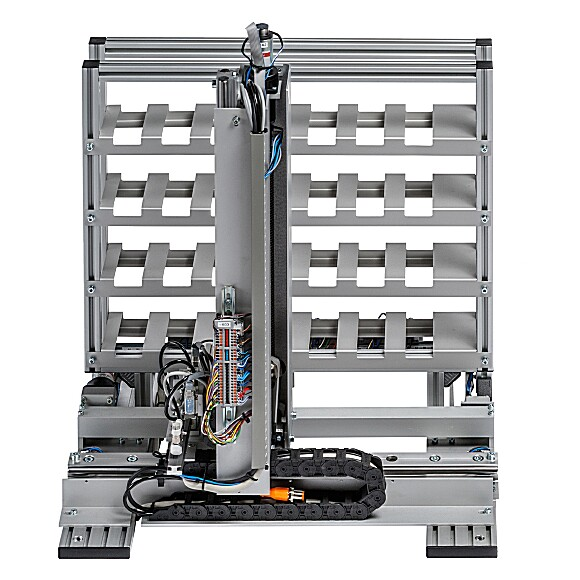
\includegraphics[width=8cm]{maquete/elevador/69523_3.jpg}
    };
    % \draw[red,ultra thick,rounded corners] (0,0) rectangle (9.4,6.2);
    \begin{scope}[x={(image.south east)},y={(image.north west)}]
        % \draw[help lines,xstep=.1,ystep=.1] (0,0) grid (1,1);
        % \foreach \x in {0,1,...,9} { \node [anchor=north] at (\x/10,0) {0.\x}; }
        % \foreach \y in {0,1,...,9} { \node [anchor=east] at (0,\y/10) {0.\y}; }
      \draw[red] (1,0.5) node {\textbf{Right}};
      \draw[red] (0,0.5) node {\textbf{Left}};
      \draw[red] (0.5,1) node {\textbf{Top}};
      \draw[red] (0.5,0) node {\textbf{Bottom}};
      \end{scope}
  \end{tikzpicture}
  \caption{Storage Unit}
\end{figure}


\begin{figure}[H]
  \centering
  \begin{tikzpicture}
    \node[anchor=south west,inner sep=0] (image) at (0,0) {
      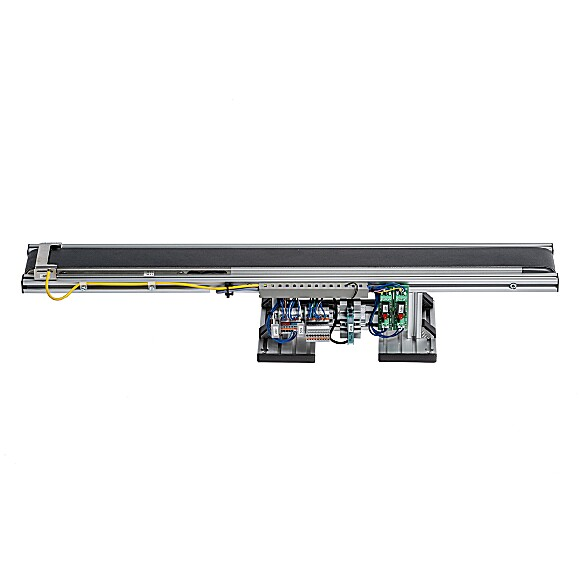
\includegraphics[trim={0 6cm 0 5cm},clip,width=8cm]{maquete/esteira/40778_3.jpg}
    };
    % \draw[red,ultra thick,rounded corners] (0,0) rectangle (9.4,6.2);
    \begin{scope}[x={(image.south east)},y={(image.north west)}]
        % \draw[help lines,xstep=.1,ystep=.1] (0,0) grid (1,1);
        % \foreach \x in {0,1,...,9} { \node [anchor=north] at (\x/10,0) {0.\x}; }
        % \foreach \y in {0,1,...,9} { \node [anchor=east] at (0,\y/10) {0.\y}; }
        \draw [->,>=stealth,red, very thick](0.9,0.7) -- (0.1,0.7);
        \draw [red] (0.5,0.8) node {Forward};
        \draw [->,>=stealth,red, very thick](0.1,0.1) -- (0.9,0.1);
        \draw [red](0.5,0.0) node {Reverse};
      \end{scope}
  \end{tikzpicture}
  \caption{Conveyor Belt}
\end{figure}

\begin{figure}[H]
  \centering
  \begin{tikzpicture}
    \node[anchor=south west,inner sep=0] (image) at (0,0) {
      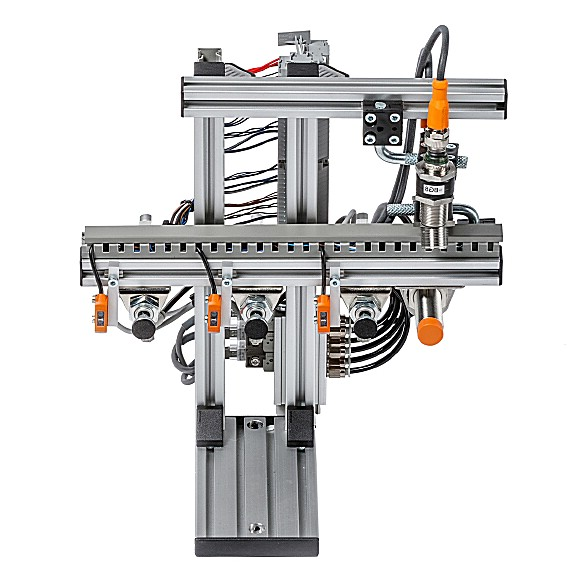
\includegraphics[trim={0 0 0 0},clip,width=8cm]{maquete/sensores/69511_3.jpg}
    };
    % \draw[red,ultra thick,rounded corners] (0,0) rectangle (9.4,6.2);
    \begin{scope}[x={(image.south east)},y={(image.north west)}]
        % \draw[help lines,xstep=.1,ystep=.1] (0,0) grid (1,1);
        % \foreach \x in {0,1,...,9} { \node [anchor=north] at (\x/10,0) {0.\x}; }
        % \foreach \y in {0,1,...,9} { \node [anchor=east] at (0,\y/10) {0.\y};  }
        \draw[red,ultra thick,rounded corners] (0.15,0.4) rectangle ++ (0.15,0.1);
        \draw[red] (0.1,0.1) node {\textbf{Left}};
        \draw[->,>=stealth,red, very thick] (0.2,0.38) -- (0.1,0.15);
        \draw[magenta,ultra thick,rounded corners] (0.35,0.4) rectangle ++ (0.15,0.1);
        \draw[magenta] (0.1,0.8) node {\textbf{Center}};
        \draw[->,>=stealth,magenta, very thick] (0.4,0.52) -- (0.2,0.75);
        \draw[cyan,ultra thick,rounded corners] (0.53,0.4) rectangle ++ (0.15,0.1);
        \draw[cyan] (0.7,0.1) node {\textbf{Right}};
        \draw[->,>=stealth,cyan, very thick] (0.65,0.38) -- (0.7,0.15);
      \end{scope}
  \end{tikzpicture}
  \caption{Sensors}
\end{figure}

\begin{figure}[H]
  \centering
  \begin{tikzpicture}
    \node[anchor=south west,inner sep=0] (image) at (0,0) {
      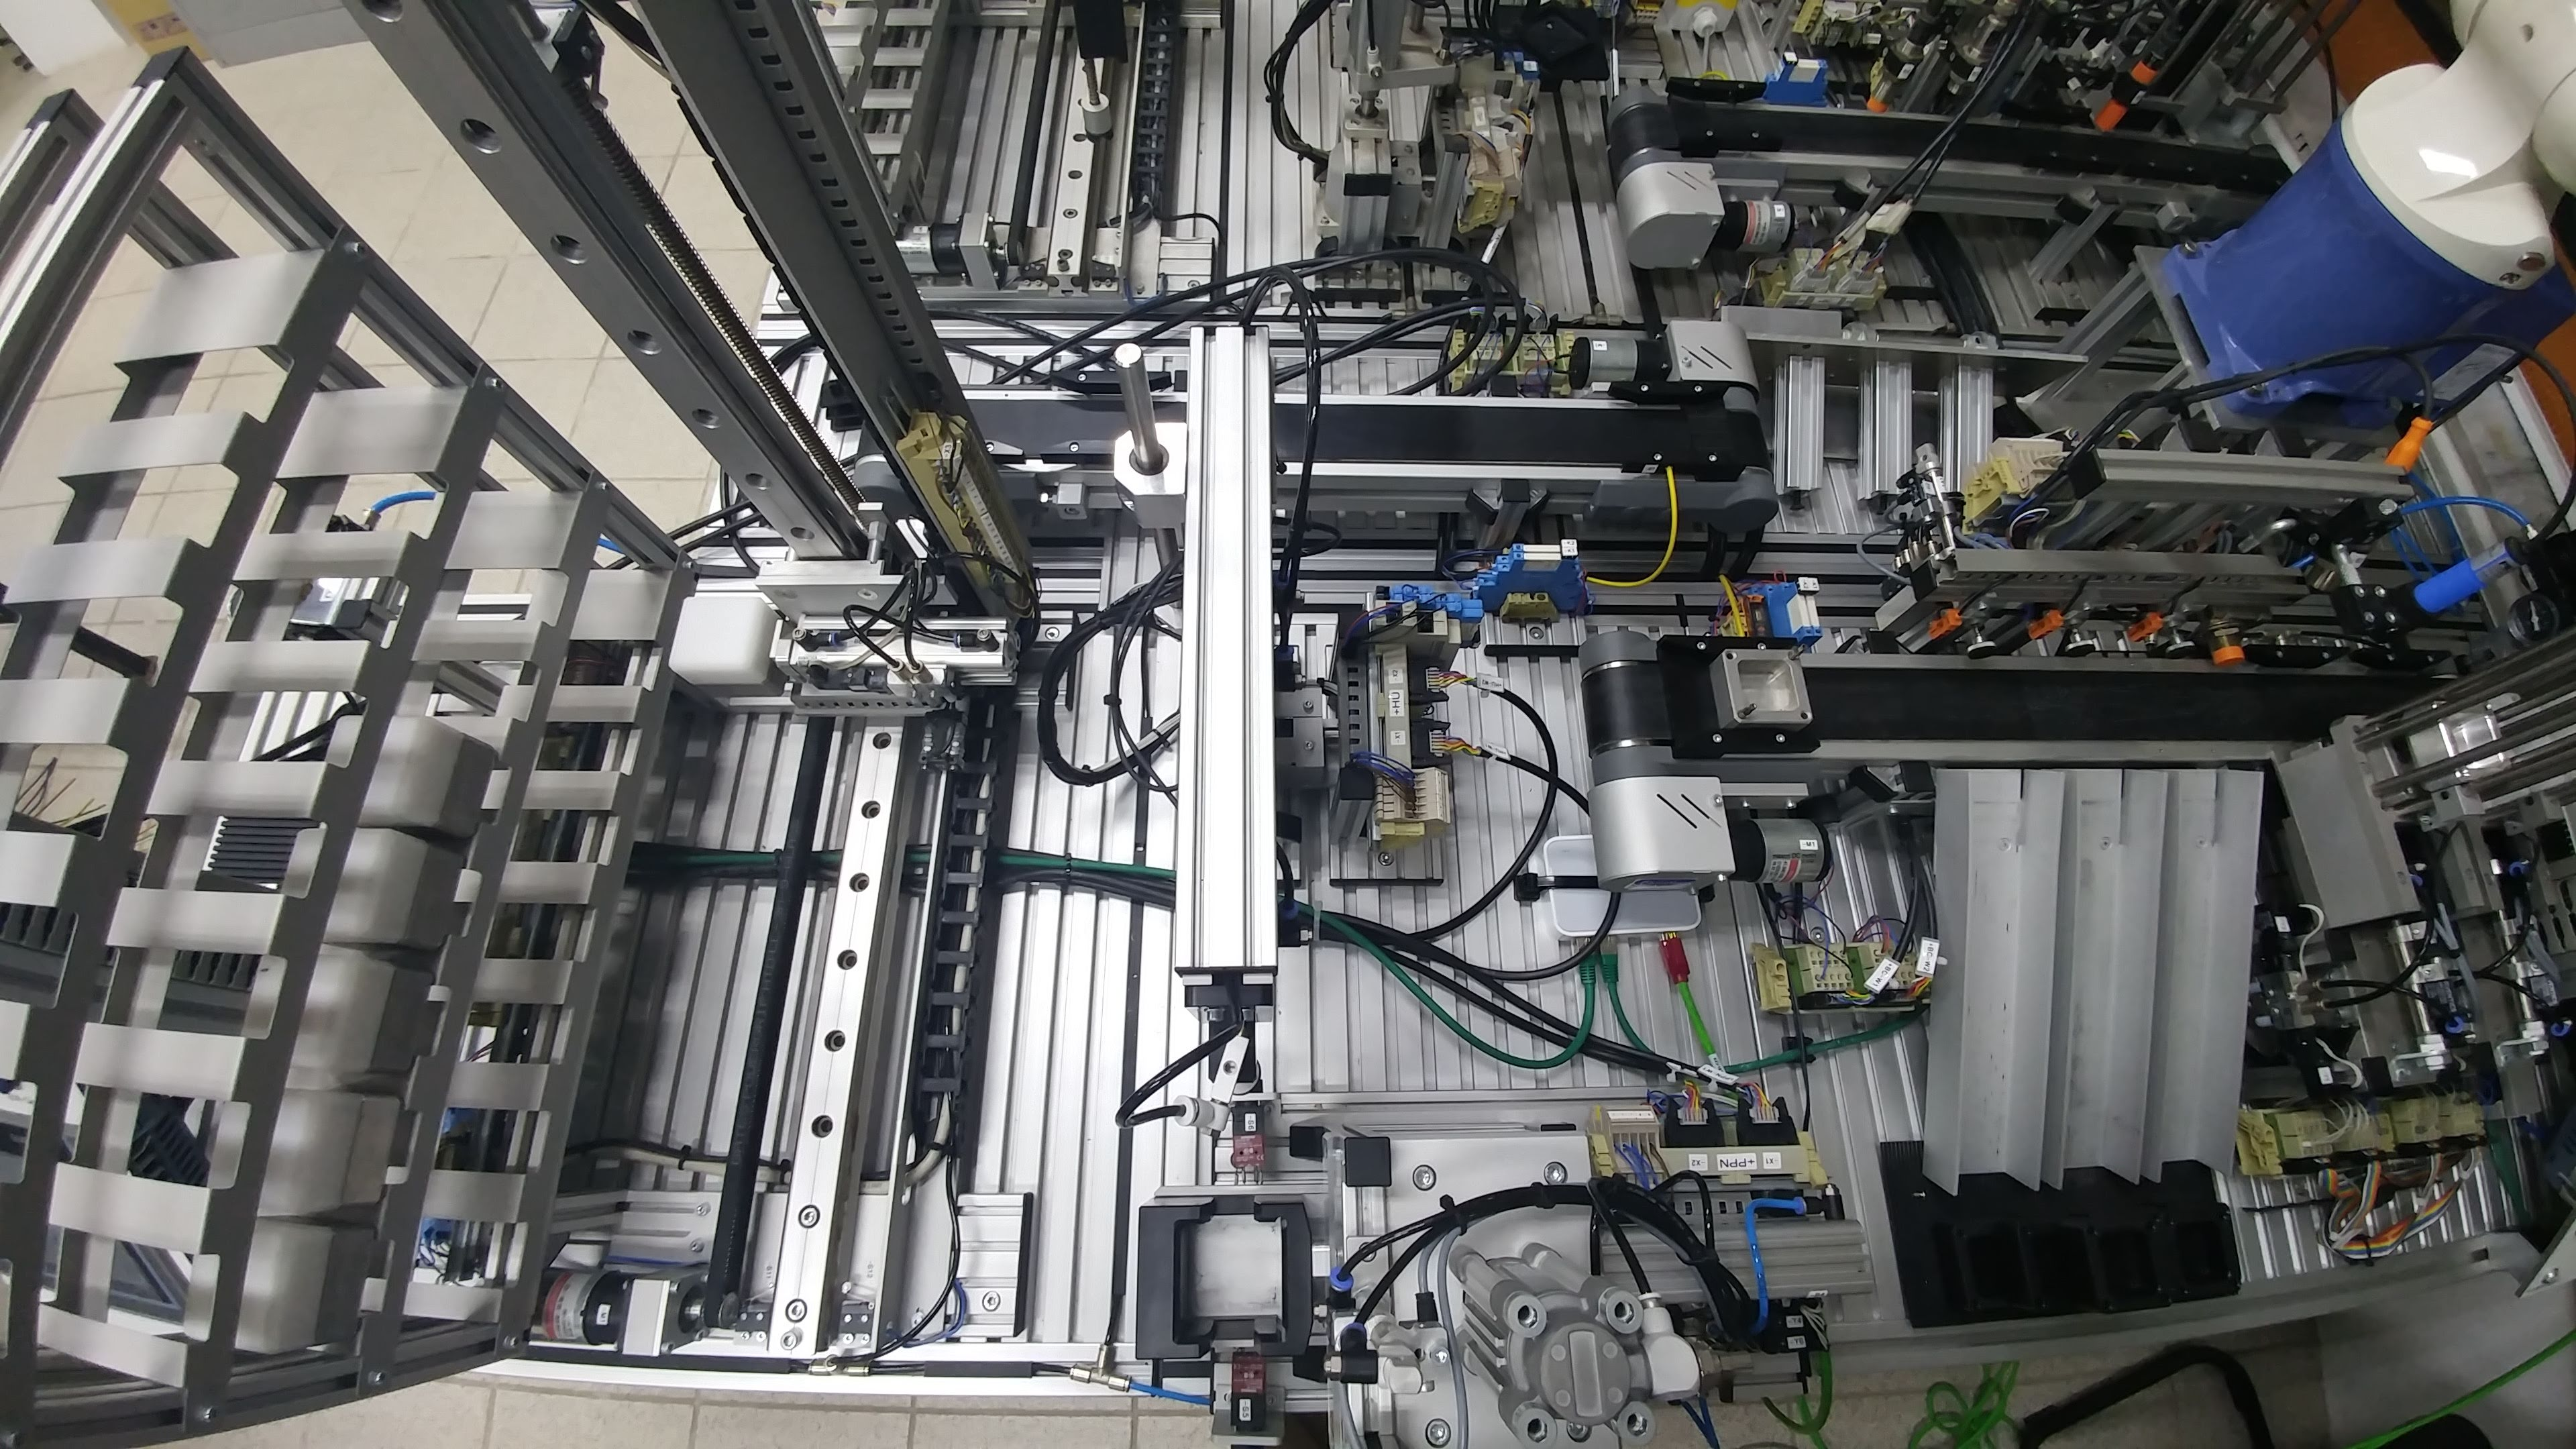
\includegraphics[trim={20cm 0 30cm 20cm},clip,width=0.8\textwidth]{maquete/armAngles.jpg}
    };
    % \draw[red,ultra thick,rounded corners] (0,0) rectangle (9.4,6.2);
    \begin{scope}[x={(image.south east)},y={(image.north west)}]
        % \draw[help lines,xstep=.1,ystep=.1] (0,0) grid (1,1);
        % \foreach \x in {0,1,...,9} { \node [anchor=north] at (\x/10,0) {0.\x}; }
        % \foreach \y in {0,1,...,9} { \node [anchor=east] at (0,\y/10) {0.\y}; }a
        
      
        \draw[red,->,>=stealth,very thick] (0.48,0.9) -- ++(-50:0.7);
        \draw[red,->,>=stealth,very thick] (0.48,0.9) -- ++(-95:0.7);
        \draw[red,->,>=stealth,very thick] (0.48,0.9) -- ++(-120:0.7);

        \draw[fill=red, fill opacity=0.2,draw=none] (0.48,0.9) -- ([shift=(-50:0.5)]0.48,0.9) arc (-50:-95:0.5);
        \draw[fill=blue, fill opacity=0.2,draw=none] (0.48,0.9) -- ([shift=(-95:0.5)]0.48,0.9) arc (-95:-120:0.5);

        \draw [fill,white,fill opacity=0.7,draw=none] (0.02,0.23) rectangle ++ (0.35,0.06);
        \draw [black] (0.2,0.25) node {\tiny \textbf{STORAGE\_ANGLE\_BEFORE}};

        \draw [fill,white,fill opacity=0.7,draw=none] (0.25,0.13) rectangle ++ (0.3,0.06);
        \draw [black] (0.4,0.15) node {\tiny \textbf{PRESS\_ANGLE\_AFTER}};

        \draw [fill,white,fill opacity=0.7,draw=none] (0.7,0.28) rectangle ++ (0.3,0.06);
        \draw [black] (0.85,0.3) node {\tiny \textbf{PRESS\_ANGLE\_BEFORE}};

        \draw [fill,white,fill opacity=0.7,draw=none] (0.1,0.82) rectangle  (0.2,0.96);
        \draw [red,thick] ([shift=(0:0.03)]0.15,0.9) arc (0:180:0.03);
        \draw[black,->,>=stealth,very thick] (0.15,0.85) -- ++(0,0.1);
        \draw [red,->,>=stealth,thick] ([shift=(0:-0.03)]0.15,0.9) arc (-180:-20:0.03);

      \end{scope}
  \end{tikzpicture}
  \caption{Sensors}
\end{figure}

Identification algorithm as seen in \cite{moreira2018enhanced}
\begin{algorithm2e}
  \caption{Identification Algorithm}\label{alg:identification}
\KwIn
{%
Modified observed paths $p_i^k$, for i= 1,\dots,$r$
}
\KwOut
{%
DAOCT = $($\XSet,\SigmaSet,\OmegaSet,\ffunction,\lambdafunction,\RSet,\thetafunction,\xZero,\XfSet$)$
}
\BlankLine
Create an initial state $x_0$, and define $\lambda(x_0) = \tilde{\lambda}(x_0) =
y_{1,1}$

$X = \{ x_0\}, X_f = \emptyset$

\For{$i = 1$ \KwTo $r$}
{
\For{$j = 1$ \KwTo $l_i - 1$}
{
  Find the State $x \in X $ such that $\tilde{\lambda}(x) = y_{i,j+1}$

  \eIf{$\tilde{\lambda}(x) \neq y_{i,j+1}$ for all $ x \in X$}
  { Create state $x^\prime$ and define $\tilde{\lambda}(x^\prime) = y_{i,j+1}$

$X = X \cup \{ x^\prime\}$

$\lambda(x^\prime) = \tilde{\lambda_l}(x^\prime)$

}
{
  Find $x^\prime \in X$ such that $\tilde{\lambda}(x^\prime) = y_{i,j+1}$
}
$f(x,\sigma_{i,j}) = x^\prime$

Add $i$ to $\theta(x,\sigma_{i,j})$

\If{$j = l_i - 1$}
{
  $X_f = X_f \cup \{x^\prime\}$
}
}
}
\end{algorithm2e}

% \begin{table}[H]
%   \centering
%   \caption{table}
%   \begin{tabular}{cc}
%     \label{tab:tab1}
%     \hypertarget{tab:1}{}
%     Transição&Significado\\
%     \hline \\
%     \hyperlink{partialNet:t1}{\hypertarget{partialTable:t1}{$t_{1}$}}&Test\\
%     \hyperlink{partialNet:p1}{\hypertarget{partialTable:p1}{$p_{1}$}}&balbalbal\\
%     \hyperlink{partialNet:p0m2}{\hypertarget{partialTable:p0m2}{$p_{0}$}}&balbalbal
%   \end{tabular}
% \end{table}

% \newpage
% \begin{figure}[h]
%   \centering
%   \begin{tikzpicture}[>=latex',line join=bevel,]
%%
\node (p0m2) at (27.0bp,18.0bp) [draw,ellipse,place, tokens=2, label=above:, label=left:\hyperlink{partialTable:p0m2}{\hypertarget{partialNet:p0m2}{$p_{0}$}},rotate=90] {};
  \node (tt1) at (114.0bp,18.0bp) [draw,ellipse,timedtransition, label=above:, label=left:\hyperlink{partialTable:tt1}{\hypertarget{partialNet:tt1}{$t_{1}$}},rotate=90] {};
  \node (ep1) at (185.0bp,18.0bp) [draw,ellipse,extPlace, label=above:, label=left:\hyperlink{partialNet:p1}{$p_{1}$},rotate=90] {};
  \draw [-Latex,inhibitor] (p0m2) ..controls (54.05bp,18.0bp) and (76.966bp,18.0bp)  .. (tt1);
  \definecolor{strokecol}{rgb}{0.0,0.0,0.0};
  \pgfsetstrokecolor{strokecol}
  \draw (70.5bp,27.0bp) node {3};
  \draw [-Latex] (tt1) ..controls (141.25bp,18.0bp) and (147.94bp,18.0bp)  .. (ep1);
%
\end{tikzpicture}

%   \caption{example }
%   \label{fig:example}
% \end{figure}

% \newpage
% \begin{figure}[h]
%   \centering
%   \begin{tikzpicture}[>=latex',line join=bevel,]
%%
\node (et1) at (27.0bp,18.0bp) [draw,ellipse,extTransition, label=above:, label=left:\hyperlink{partialNet:t1}{$t_{1}$},rotate=90] {};
  \node (p1) at (95.0bp,18.0bp) [draw,ellipse,place, label=above:, label=left:\hyperlink{partialTable:p1}{\hypertarget{partialNet:p1}{$p_{1}$}},rotate=90] {};
  \draw [-Latex] (et1) ..controls (54.266bp,18.0bp) and (57.727bp,18.0bp)  .. (p1);
%
\end{tikzpicture}

%   \caption{example }
%   \label{fig:example}
% \end{figure}

% \newpage

% \begin{figure}[H]
%   \centering
%   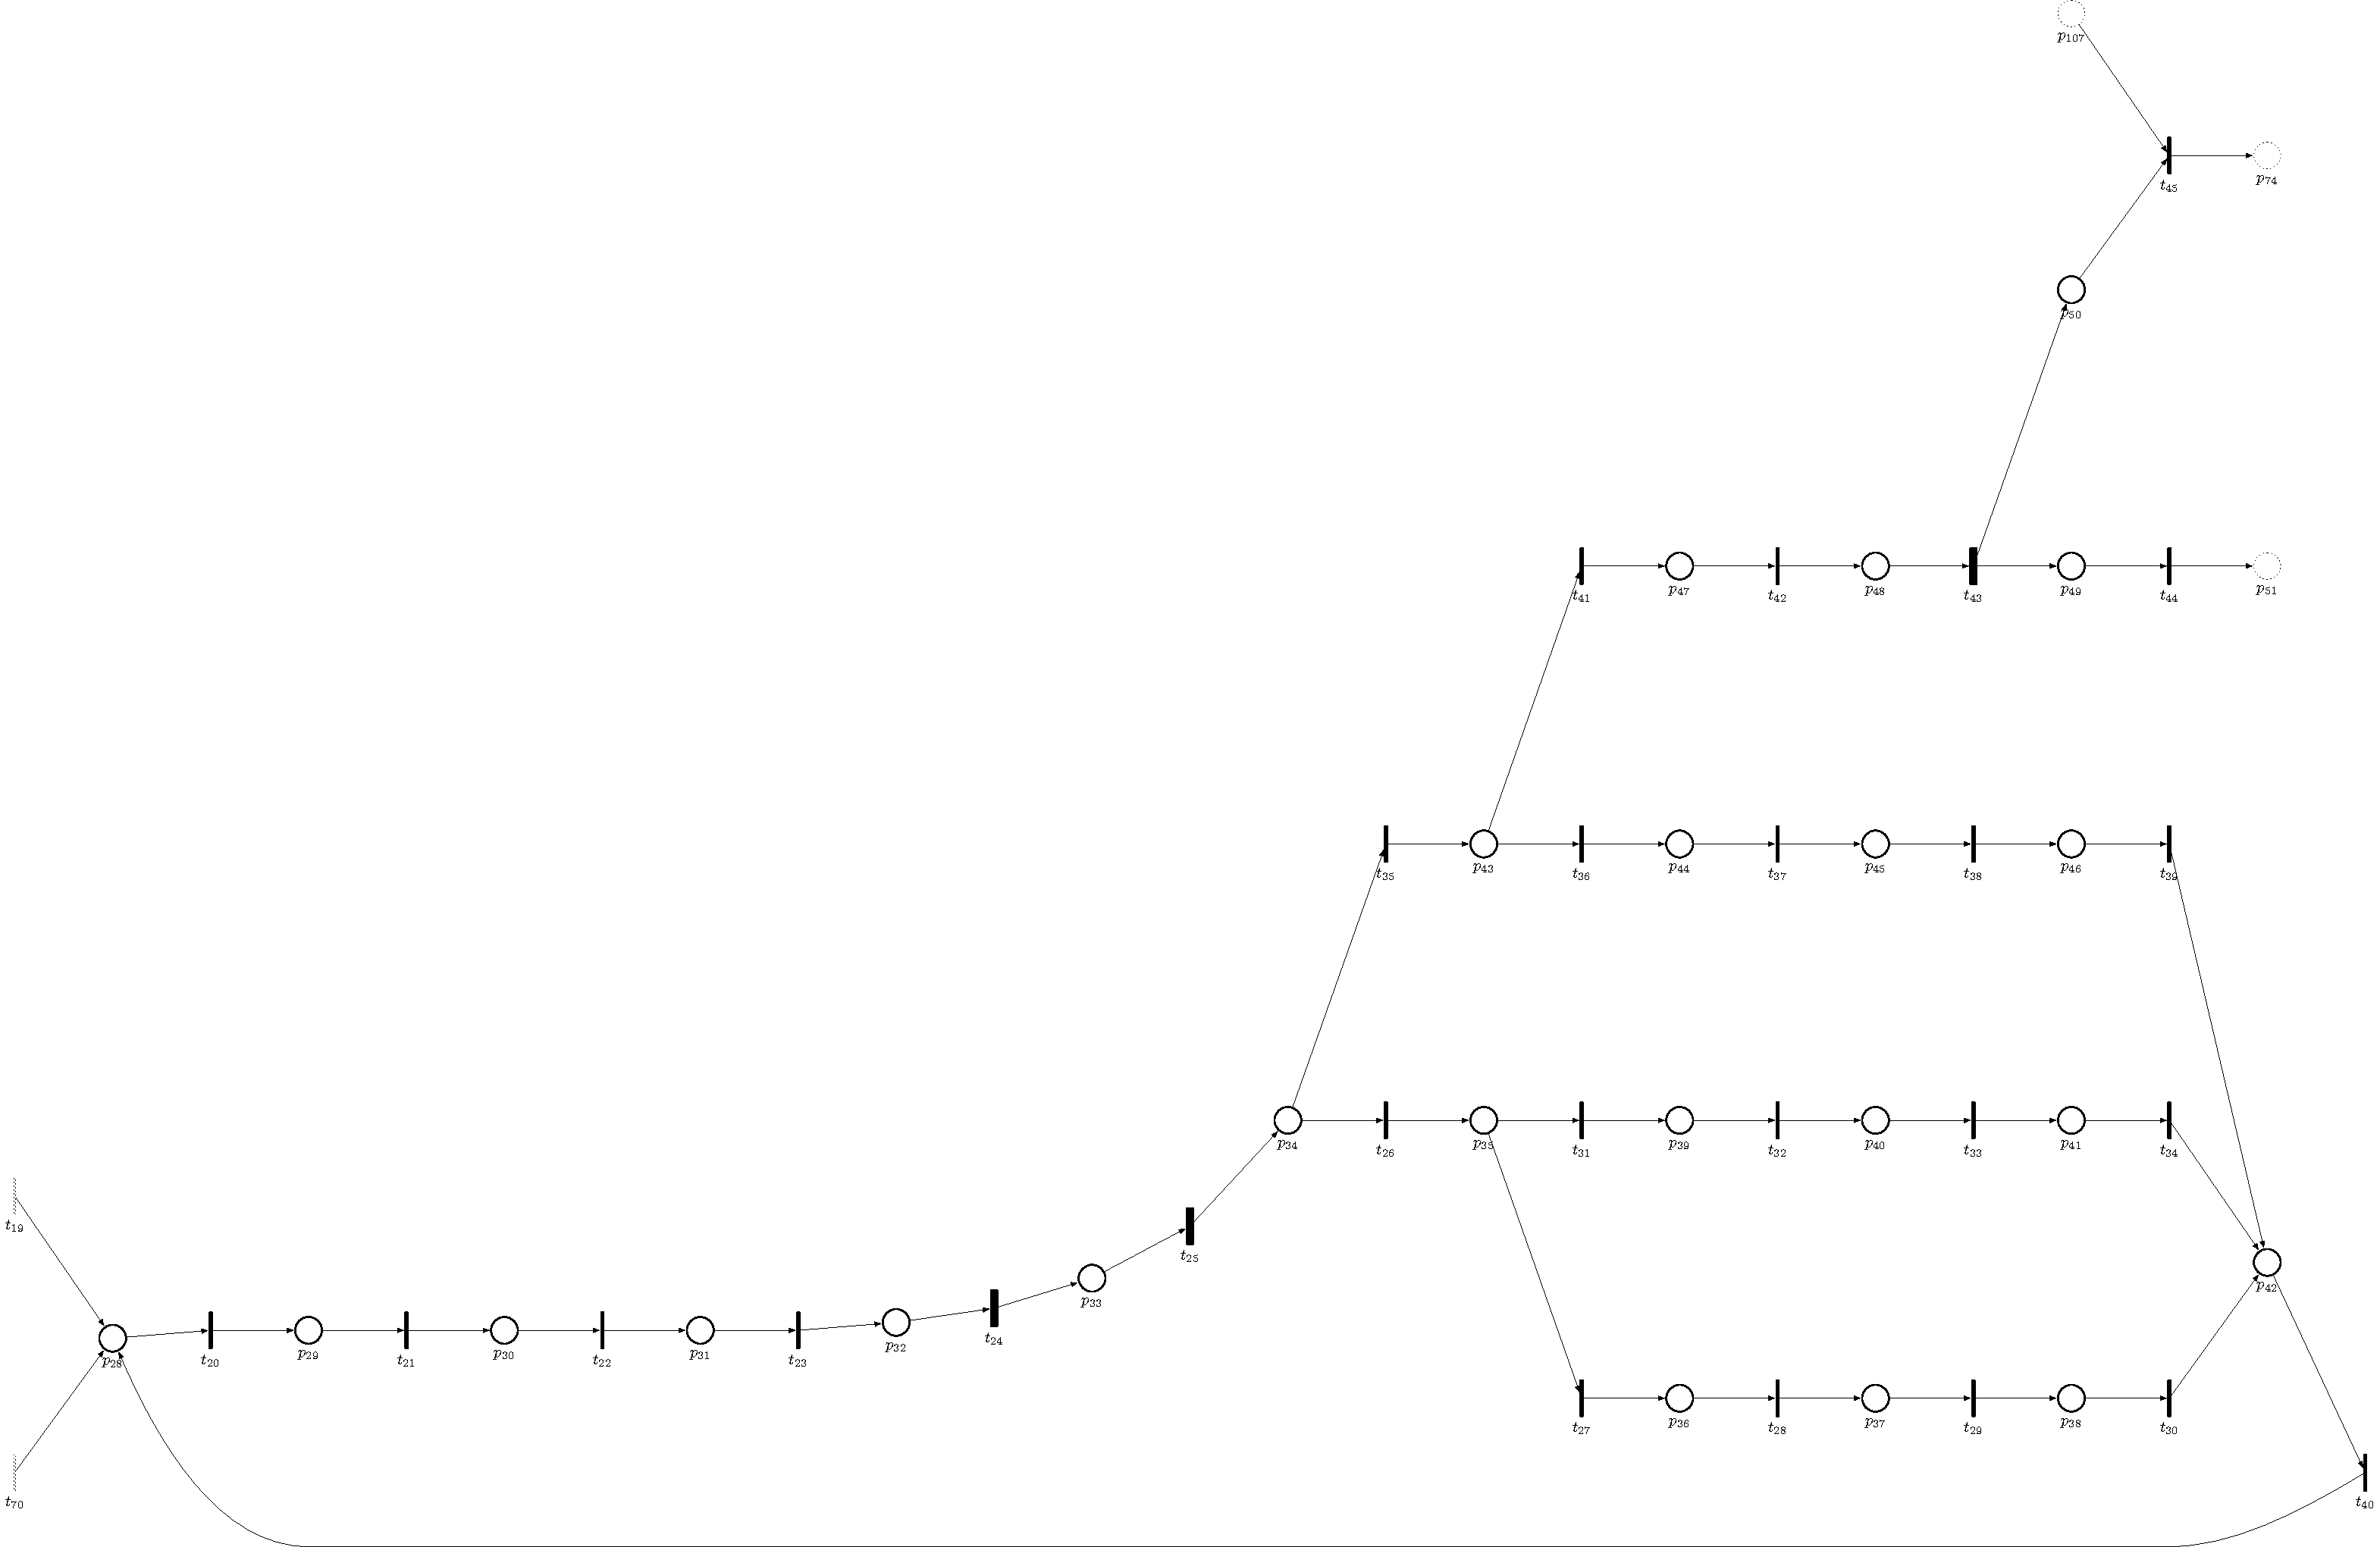
\includegraphics{../../figures/petriNet/dot/2-metalv/metalv.pdf}
%   \caption{qlksdjf}
%   \label{fig:example}
% \end{figure}


% \begin{figure}[H]
%   \centering
%   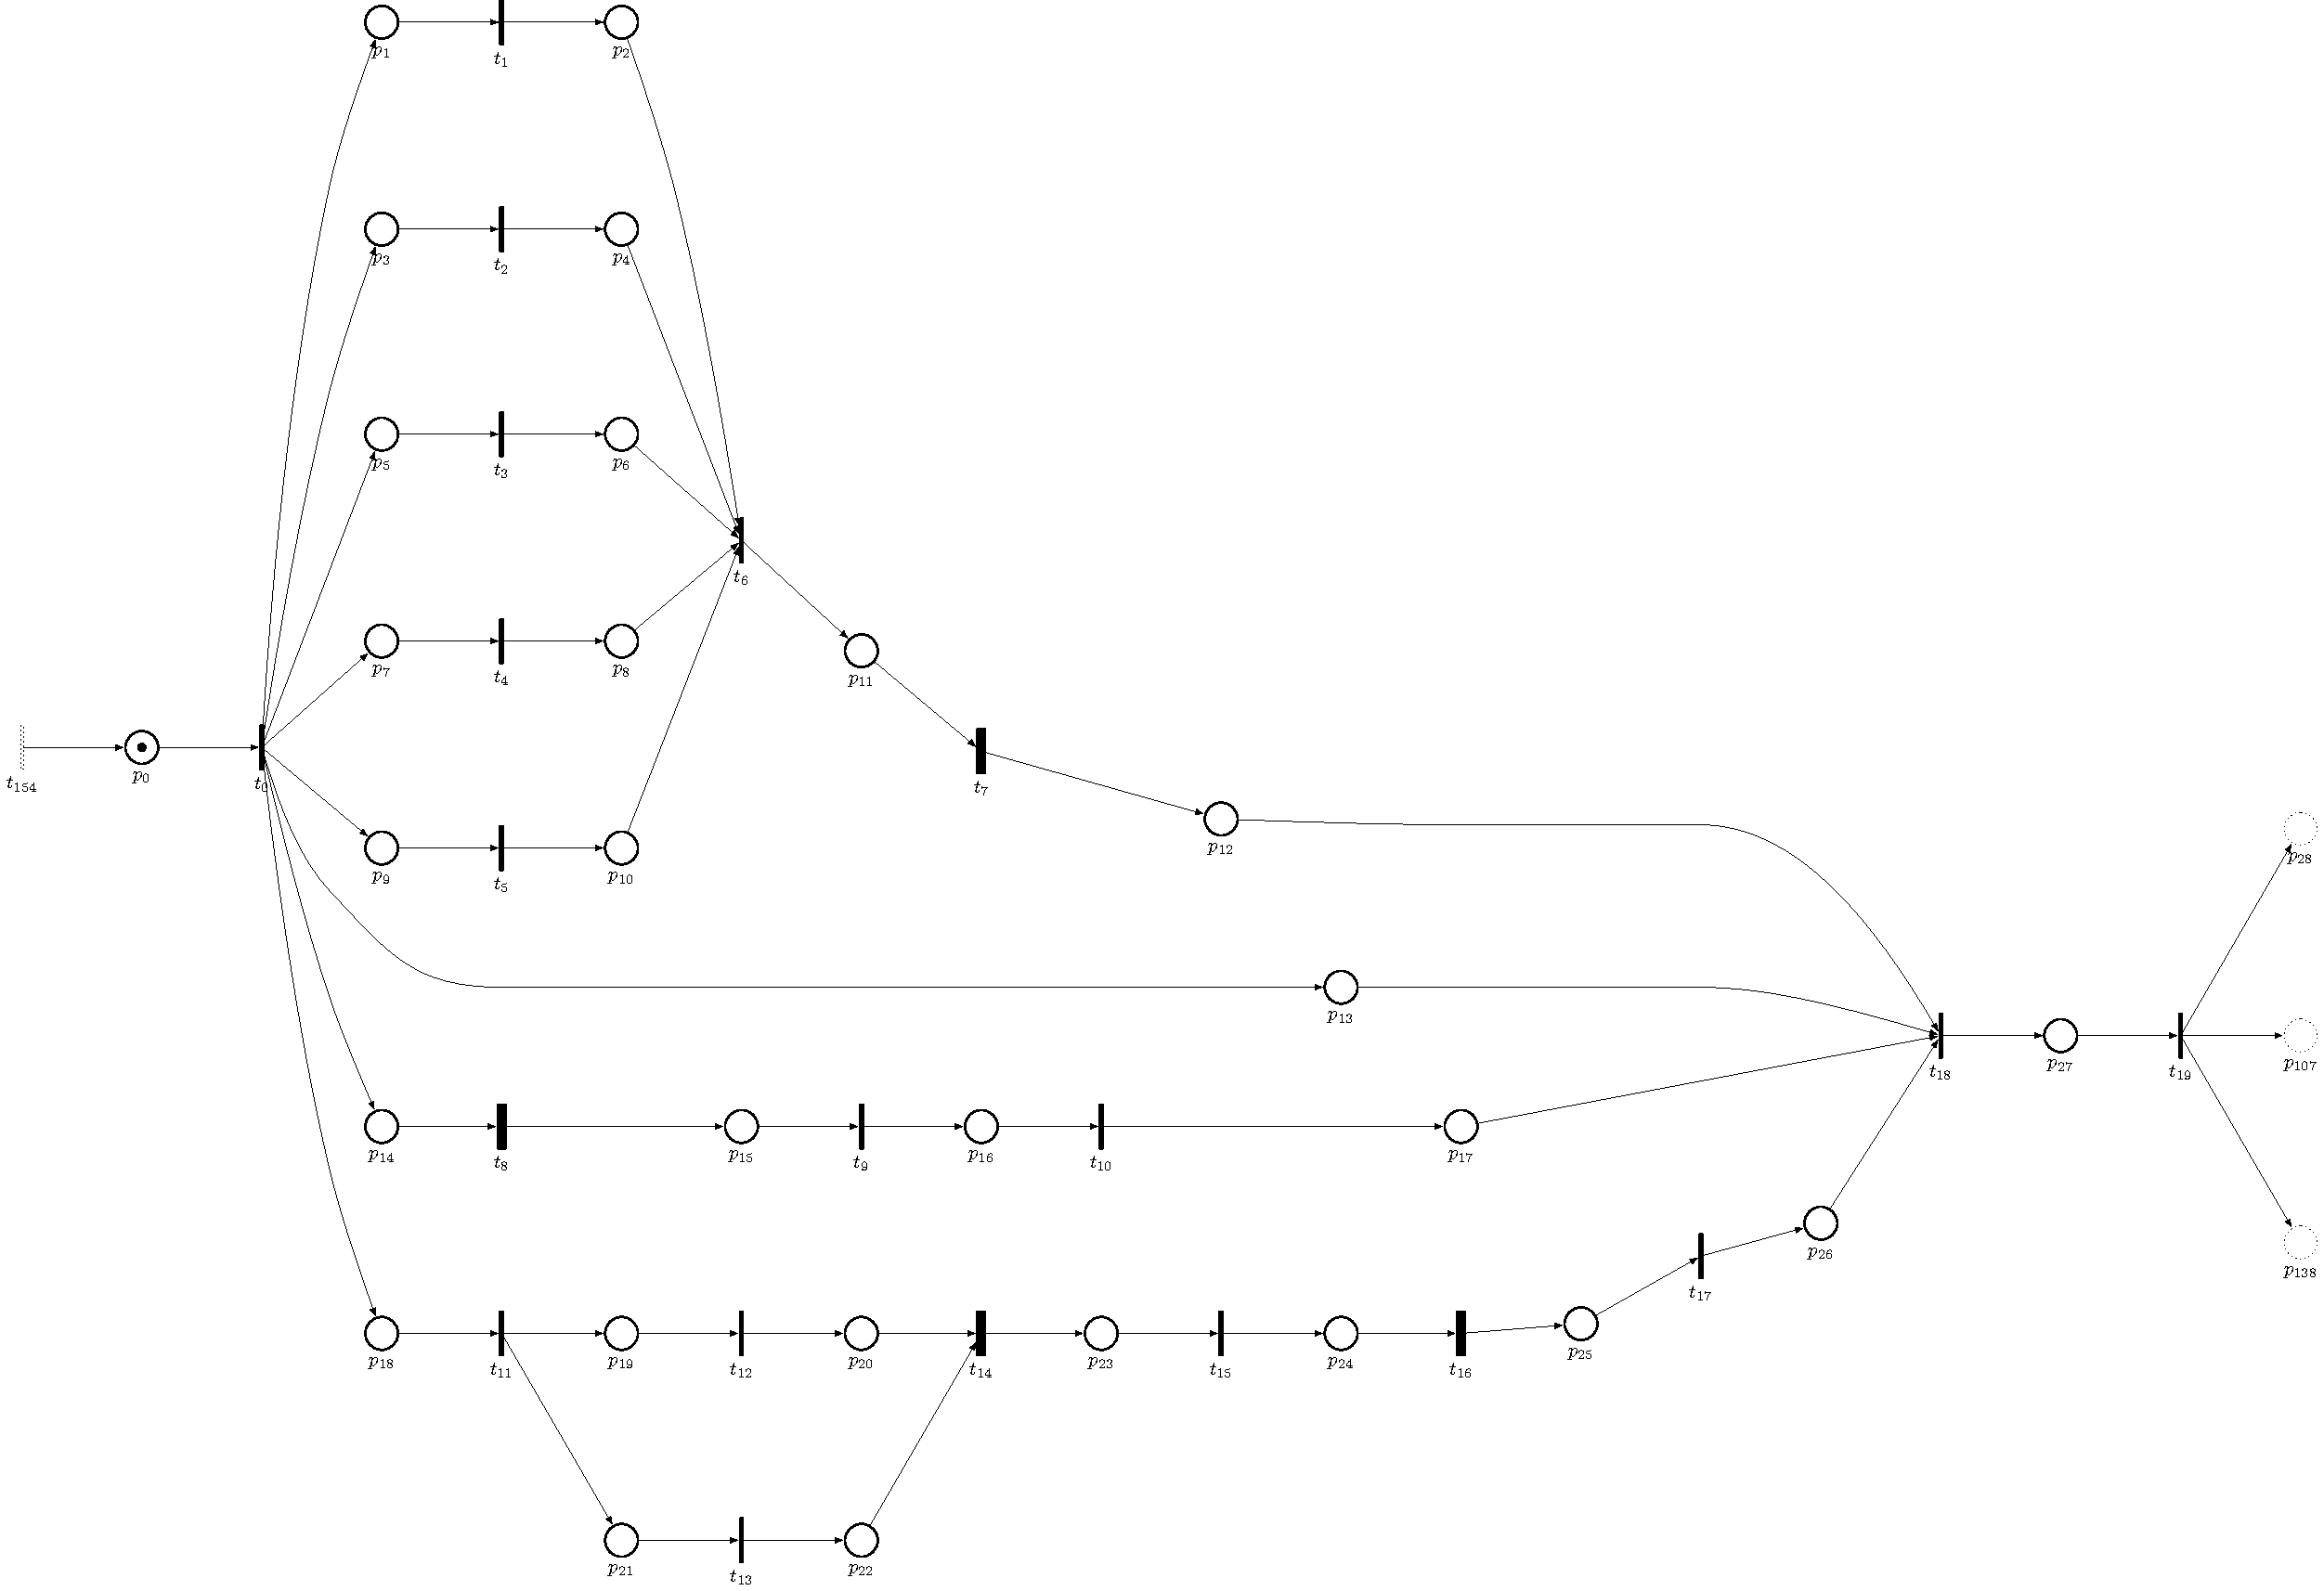
\includegraphics[width=0.4\textwidth]{../../figures/partial/initial.tikz}
%   \caption{petri net bal}
%   \label{fig:petrinetexample}
% \end{figure}

% \addtikzfigure{../../figures/petriNet/partial/initial}
% {Petri net of cube storage module.}
% {petri_initialization}

% \addtikzfigure{../../figures/petriNet//partial/metalv}
% {Petri net of metal cube half sorting module.}
% {petri_initialization}

\begin{table}[htbp]
\caption{Initialization Module Places.}
\centering
\begin{tabular}{M{5cm}M{10cm}}
Places & Meaning\\
\hline
\hyperlink{partialNet:p0m1}{\hypertarget{partialTable:p0m1}{$p_{0}$}} & System Stopped\\
\hyperlink{partialNet:p1}{\hypertarget{partialTable:p1}{$p_{1}$}} & Retract MAG1's Cylinder *\\
\hyperlink{partialNet:p2}{\hypertarget{partialTable:p2}{$p_{2}$}} & MAG1's Cylinder Retracted\\
\hyperlink{partialNet:p3}{\hypertarget{partialTable:p3}{$p_{3}$}} & Retract MAG2's Cylinder *\\
\hyperlink{partialNet:p4}{\hypertarget{partialTable:p4}{$p_{4}$}} & MAG2's Cylinder Retracted\\
\hyperlink{partialNet:p5}{\hypertarget{partialTable:p5}{$p_{5}$}} & Retract Right Discharge Cylinder *\\
\hyperlink{partialNet:p6}{\hypertarget{partialTable:p6}{$p_{6}$}} & Right Discharge Cylinder Retracted\\
\hyperlink{partialNet:p7}{\hypertarget{partialTable:p7}{$p_{7}$}} & Retract Center Discharge Cylinder\\
\hyperlink{partialNet:p8}{\hypertarget{partialTable:p8}{$p_{8}$}} & Center Discharge Cylinder Retracted\\
\hyperlink{partialNet:p9}{\hypertarget{partialTable:p9}{$p_{9}$}} & Retract Left Discharge Cylinder *\\
\hyperlink{partialNet:p10}{\hypertarget{partialTable:p10}{$p_{10}$}} & Left Discharge Cylinder Retracted\\
\hyperlink{partialNet:p11}{\hypertarget{partialTable:p11}{$p_{11}$}} & Turn Conveyor Belt On (Reverse)\\
\hyperlink{partialNet:p12}{\hypertarget{partialTable:p12}{$p_{12}$}} & No Pieces On Conveyor Belt\\
\hyperlink{partialNet:p13}{\hypertarget{partialTable:p13}{$p_{13}$}} & Reset Variables\\
\hyperlink{partialNet:p14}{\hypertarget{partialTable:p14}{$p_{14}$}} & Raise Press\\
\hyperlink{partialNet:p15}{\hypertarget{partialTable:p15}{$p_{15}$}} & Open Safety Door\\
\hyperlink{partialNet:p16}{\hypertarget{partialTable:p16}{$p_{16}$}} & Extend Assembly Unit Holder\\
\hyperlink{partialNet:p17}{\hypertarget{partialTable:p17}{$p_{17}$}} & Assembly Unit Ready\\
\hyperlink{partialNet:p18}{\hypertarget{partialTable:p18}{$p_{18}$}} & Arm Lowered and Retracted, and Storage Unit Retracted\\
\hyperlink{partialNet:p19}{\hypertarget{partialTable:p19}{$p_{19}$}} & Move Storage Unit to the Right\\
\hyperlink{partialNet:p20}{\hypertarget{partialTable:p20}{$p_{20}$}} & Storage Unit ready ( horizontal )\\
\hyperlink{partialNet:p21}{\hypertarget{partialTable:p21}{$p_{21}$}} & Move Storage Device Downwards\\
\hyperlink{partialNet:p22}{\hypertarget{partialTable:p22}{$p_{22}$}} & Storage Unit ready ( vertical )\\
\hyperlink{partialNet:p23}{\hypertarget{partialTable:p23}{$p_{23}$}} & Rotate Arm CCW\\
\hyperlink{partialNet:p24}{\hypertarget{partialTable:p24}{$p_{24}$}} & Turn HSC Off ( Arm Stopped )\\
\hyperlink{partialNet:p25}{\hypertarget{partialTable:p25}{$p_{25}$}} & Rotate Arm CW\\
\hyperlink{partialNet:p26}{\hypertarget{partialTable:p26}{$p_{26}$}} & Arm Stopped facing conveyor belt\\
\hyperlink{partialNet:p27}{\hypertarget{partialTable:p27}{$p_{27}$}} & System Ready\\
\end{tabular}
\end{table}


\begin{table}[H]
\caption{Initialization Module Transitions.}
\centering
\begin{tabular}{M{5cm}M{10cm}}
Transitions & Meaning\\
\hline
\hyperlink{partialNet:t0}{\hypertarget{partialTable:t0}{$t_{0}$}} & Initialization Button\\
\hyperlink{partialNet:t1}{\hypertarget{partialTable:t1}{$t_{1}$}} & MAG1's Cylinder Retracted\\
\hyperlink{partialNet:t2}{\hypertarget{partialTable:t2}{$t_{2}$}} & MAG2's Cylinder Retracted\\
\hyperlink{partialNet:t3}{\hypertarget{partialTable:t3}{$t_{3}$}} & Right Discharge Cylinder Retracted\\
\hyperlink{partialNet:t4}{\hypertarget{partialTable:t4}{$t_{4}$}} & Center Discharge Cylinder Retracted\\
\hyperlink{partialNet:t5}{\hypertarget{partialTable:t5}{$t_{5}$}} & Left Discharge Cylinder Retracted\\
\hyperlink{partialNet:t6}{\hypertarget{partialTable:t6}{$t_{6}$}} & \\
\hyperlink{partialNet:tt7}{\hypertarget{partialTable:tt7}{$t_{7}$}} & T=12s\\
\hyperlink{partialNet:tt8}{\hypertarget{partialTable:tt8}{$t_{8}$}} & T=2.5s\\
\hyperlink{partialNet:t9}{\hypertarget{partialTable:t9}{$t_{9}$}} & Safety Door Opened\\
\hyperlink{partialNet:t10}{\hypertarget{partialTable:t10}{$t_{10}$}} & Assembly Unit Holder Extended\\
\hyperlink{partialNet:t11}{\hypertarget{partialTable:t11}{$t_{11}$}} & Storage Unit Retracted and Arm Lowered and Retracted\\
\hyperlink{partialNet:t12}{\hypertarget{partialTable:t12}{$t_{12}$}} & Storage Unit Right Limit Switch\\
\hyperlink{partialNet:t13}{\hypertarget{partialTable:t13}{$t_{13}$}} & Storage Unit Inferior Limit Switch\\
\hyperlink{partialNet:tt14}{\hypertarget{partialTable:tt14}{$t_{14}$}} & T=2s\\
\hyperlink{partialNet:t15}{\hypertarget{partialTable:t15}{$t_{15}$}} & Inductive Sensor Arm\\
\hyperlink{partialNet:tt16}{\hypertarget{partialTable:tt16}{$t_{16}$}} & T=1s\\
\hyperlink{partialNet:t17}{\hypertarget{partialTable:t17}{$t_{17}$}} & ARMCOUNTER <= BELT\_ANGLE\_CW\\
\hyperlink{partialNet:t18}{\hypertarget{partialTable:t18}{$t_{18}$}} & \\
\hyperlink{partialNet:t19}{\hypertarget{partialTable:t19}{$t_{19}$}} & Start Button\\
\end{tabular}
\end{table}


\begin{longtable}{M{5cm}M{10cm}}
\caption{Metal Half-cube Selection Module Places.} \label{tab:metalvPlaces}
\\
Places & Meaning\\
\hline
\endfirsthead
\multicolumn{2}{l}{Continued from previous page} \\
\hline

Places & Meaning \\

\hline
\endhead
\hline\multicolumn{2}{r}{Continued on next page} \\
\endfoot
\endlastfoot
\hline
\hyperlink{partialNet:p28}{\hypertarget{partialTable:p28}{$p_{28}$}} & MAG1 Empty\\
\hyperlink{partialNet:p29}{\hypertarget{partialTable:p29}{$p_{29}$}} & MAG1 Not Empty\\
\hyperlink{partialNet:p30}{\hypertarget{partialTable:p30}{$p_{30}$}} & Extend MAG1's Cylinder *\\
\hyperlink{partialNet:p31}{\hypertarget{partialTable:p31}{$p_{31}$}} & Retract MAG1's Cylinder *\\
\hyperlink{partialNet:p32}{\hypertarget{partialTable:p32}{$p_{32}$}} & MAG1's Cylinder Retracted\\
\hyperlink{partialNet:p33}{\hypertarget{partialTable:p33}{$p_{33}$}} & Turn Conveyor Belt On\\
\hyperlink{partialNet:p34}{\hypertarget{partialTable:p34}{$p_{34}$}} & \\
\hyperlink{partialNet:p35}{\hypertarget{partialTable:p35}{$p_{35}$}} & Plastic Half-cube\\
\hyperlink{partialNet:p36}{\hypertarget{partialTable:p36}{$p_{36}$}} & Turn Conveyor Belt On\\
\hyperlink{partialNet:p37}{\hypertarget{partialTable:p37}{$p_{37}$}} & Extend Right Discharge Cylinder *\\
\hyperlink{partialNet:p38}{\hypertarget{partialTable:p38}{$p_{38}$}} & Retract Right Discharge Cylinder *\\
\hyperlink{partialNet:p39}{\hypertarget{partialTable:p39}{$p_{39}$}} & Turn Conveyor Belt On\\
\hyperlink{partialNet:p40}{\hypertarget{partialTable:p40}{$p_{40}$}} & Extend Center Discharge Cylinder *\\
\hyperlink{partialNet:p41}{\hypertarget{partialTable:p41}{$p_{41}$}} & Retract Center Discharge Cylinder *\\
\hyperlink{partialNet:p42}{\hypertarget{partialTable:p42}{$p_{42}$}} & \\
\hyperlink{partialNet:p43}{\hypertarget{partialTable:p43}{$p_{43}$}} & Metal Half-cube\\
\hyperlink{partialNet:p44}{\hypertarget{partialTable:p44}{$p_{44}$}} & Turn Conveyor Belt On\\
\hyperlink{partialNet:p45}{\hypertarget{partialTable:p45}{$p_{45}$}} & Extend Left Discharge Cylinder *\\
\hyperlink{partialNet:p46}{\hypertarget{partialTable:p46}{$p_{46}$}} & Retract Left Discharge Cylinder *\\
\hyperlink{partialNet:p47}{\hypertarget{partialTable:p47}{$p_{47}$}} & Turn Conveyor Belt On\\
\hyperlink{partialNet:p48}{\hypertarget{partialTable:p48}{$p_{48}$}} & Turn Conveyor Belt On\\
\hyperlink{partialNet:p49}{\hypertarget{partialTable:p49}{$p_{49}$}} & Metal Half-cube Ready\\
\hyperlink{partialNet:p50}{\hypertarget{partialTable:p50}{$p_{50}$}} & Conveyor Belt Stopped\\
\end{longtable}


\begin{table}[H]
\caption{Metal Half-cube Selection Module Transitions.}
\centering
\begin{tabular}{M{5cm}M{10cm}}
Transitions & Meaning\\
\hline
\hyperlink{partialNet:t20}{\hypertarget{partialTable:t20}{$t_{20}$}} & \(\overline{\mbox{MAG1 Empty}}\)\\
\hyperlink{partialNet:t21}{\hypertarget{partialTable:t21}{$t_{21}$}} & \\
\hyperlink{partialNet:t22}{\hypertarget{partialTable:t22}{$t_{22}$}} & MAG1's Cylinder Extended \(\uparrow\)\\
\hyperlink{partialNet:t23}{\hypertarget{partialTable:t23}{$t_{23}$}} & MAG1's Cylinder Retracted \(\uparrow\)\\
\hyperlink{partialNet:tt24}{\hypertarget{partialTable:tt24}{$t_{24}$}} & T=0.5s\\
\hyperlink{partialNet:tt25}{\hypertarget{partialTable:tt25}{$t_{25}$}} & Presence \(\uparrow\) T=0.5s\\
\hyperlink{partialNet:t26}{\hypertarget{partialTable:t26}{$t_{26}$}} & \(\overline{\mbox{Metallic Sensor}}\)\\
\hyperlink{partialNet:t27}{\hypertarget{partialTable:t27}{$t_{27}$}} & \(\overline{\mbox{White Color Sensor}}\)\\
\hyperlink{partialNet:t28}{\hypertarget{partialTable:t28}{$t_{28}$}} & Proximity Sensor Left Discharge Cylinder \(\uparrow\)\\
\hyperlink{partialNet:t29}{\hypertarget{partialTable:t29}{$t_{29}$}} & Right Discharge Cylinder Extended\\
\hyperlink{partialNet:t30}{\hypertarget{partialTable:t30}{$t_{30}$}} & Right Discharge Cylinder Retracted\\
\hyperlink{partialNet:t31}{\hypertarget{partialTable:t31}{$t_{31}$}} & White Color Sensor\\
\hyperlink{partialNet:t32}{\hypertarget{partialTable:t32}{$t_{32}$}} & Proximity Sensor Center Discharge Cylinder \(\uparrow\)\\
\hyperlink{partialNet:t33}{\hypertarget{partialTable:t33}{$t_{33}$}} & Center Discharge Cylinder Extended\\
\hyperlink{partialNet:t34}{\hypertarget{partialTable:t34}{$t_{34}$}} & Center Discharge Cylinder Retracted\\
\hyperlink{partialNet:t35}{\hypertarget{partialTable:t35}{$t_{35}$}} & Metallic Sensor\\
\hyperlink{partialNet:t36}{\hypertarget{partialTable:t36}{$t_{36}$}} & Concavity Downwards\\
\hyperlink{partialNet:t37}{\hypertarget{partialTable:t37}{$t_{37}$}} & Proximity Sensor Left Discharge Cylinder \(\uparrow\)\\
\hyperlink{partialNet:t38}{\hypertarget{partialTable:t38}{$t_{38}$}} & Left Discharge Cylinder Extended\\
\hyperlink{partialNet:t39}{\hypertarget{partialTable:t39}{$t_{39}$}} & Left Discharge Cylinder Retracted\\
\hyperlink{partialNet:t40}{\hypertarget{partialTable:t40}{$t_{40}$}} & \\
\hyperlink{partialNet:t41}{\hypertarget{partialTable:t41}{$t_{41}$}} & Concavity Upwards\\
\hyperlink{partialNet:t42}{\hypertarget{partialTable:t42}{$t_{42}$}} & Proximity Sensor End Of Conveyor Belt \(\uparrow\)\\
\hyperlink{partialNet:tt43}{\hypertarget{partialTable:tt43}{$t_{43}$}} & T=0.5s\\
\hyperlink{partialNet:t44}{\hypertarget{partialTable:t44}{$t_{44}$}} & Proximity Sensor End Of Conveyor Belt \(\downarrow\)\\
\hyperlink{partialNet:t45}{\hypertarget{partialTable:t45}{$t_{45}$}} & \\
\end{tabular}
\end{table}


%%% Local Variables:
%%% mode: latex
%%% TeX-master: "../monografia"
%%% End:
